\documentclass[11pt]{aghdpl}
% \documentclass[en,11pt]{aghdpl}  % praca w języku angielskim
\usepackage[polish]{babel}
%\usepackage[english]{babel}
\usepackage[utf8]{inputenc}

% dodatkowe pakiety
\usepackage{enumerate}
\usepackage{listings}
\lstloadlanguages{TeX}

\lstset{
  literate={ą}{{\k{a}}}1
           {ć}{{\'c}}1
           {ę}{{\k{e}}}1
           {ó}{{\'o}}1
           {ń}{{\'n}}1
           {ł}{{\l{}}}1
           {ś}{{\'s}}1
           {ź}{{\'z}}1
           {ż}{{\.z}}1
           {Ą}{{\k{A}}}1
           {Ć}{{\'C}}1
           {Ę}{{\k{E}}}1
           {Ó}{{\'O}}1
           {Ń}{{\'N}}1
           {Ł}{{\L{}}}1
           {Ś}{{\'S}}1
           {Ź}{{\'Z}}1
           {Ż}{{\.Z}}1
}

%---------------------------------------------------------------------------

\author{Rafał Włodarz}
\shortauthor{R. Włodarz}

\titlePL{Algorytm sterowania wykorzystujący sztuczne sieci neuronowe dla bezzałogowego statku latającego typu TRICOPTER}
\titleEN{}

\shorttitlePL{Algorytm sterowania wykorzystujący sztuczne sieci neuronowe} % skrócona wersja tytułu jeśli jest bardzo długi
%\shorttitleEN{Thesis in \LaTeX}

\thesistype{Praca dyplomowa magisterska}
%\thesistype{Master of Science Thesis}

\supervisor{dr hab. Adam Piłat}
%\supervisor{Marcin Szpyrka PhD, DSc}

\degreeprogramme{Automatyka i robotyka}
%\degreeprogramme{Computer Science}

\date{2015}

\department{Katedra Automatyki}
%\department{Department of Applied Computer Science}

\faculty{Wydział Elektrotechniki, Automatyki,\protect\\[-1mm] Informatyki i Inżynierii Biomedycznej}
%\faculty{Faculty of Electrical Engineering, Automatics, Computer Science and Biomedical Engineering}

\acknowledgements{Serdecznie dziękuję \dots tu ciąg dalszych podziękowań np. dla promotora, żony, sąsiada itp.}


\setlength{\cftsecnumwidth}{10mm}

%---------------------------------------------------------------------------
\setcounter{secnumdepth}{4}

\begin{document}

\titlepages
\setcounter{tocdepth}{3}
\tableofcontents
\clearpage

\chapter{Wstęp}
\label{cha:wprowadzenie}

\section{Cele pracy}
\label{sec:celePracy}

\section{Zawartość pracy}
\label{sec: zawartosc_pracy}



















\chapter{Sztuczne sieci neuronowe}
\label{cha:sztuczne_sieci_neuronowe}

Rozdział ten zawiera informacje na temat sieci neuronowych, ich architektury, zasady działania oraz algorytmów uczenia.

\section{Początki sieci neuronowych}
\label{sec:poczatki_sieci_neuronowych}
Początki prac nad poznaniem procesów zachodzących w mózgu datuje się na rok 1943. W pracy McCulloch'a oraz Pitts'a przedstawiono matematyczny model neuronu, który zapoczątkował badania związane z tym tematem. W 1949 roku Donald Hebb odkrył, iż informacje przechowywane w sieci neuronowej są reprezentowane jako wartości wag pomiędzy poszczególnymi neuronami. Na podstawie tych informacji zaproponował on pierwszy algorytm uczenia sieci neuronowej, który został nazwany regułą Hebba. Już wtedy odkryto, iż bardzo dużą zaletą sieci jest równoległy sposób przetwarzania informacji oraz metodologia uczenia, która zastępuje tradycyjny proces programowania. 



\chapter{Architektura statku latającego typu tricopter}
\label{cha:architektura_statku_latajacego_typu_tricopter}

Poniższy rozdział przedstawia zbiór podstawowych zagadnień związanych z konstrukcją wirnikowca typu tricoper oraz zawiera informacje na temat zasad sterowania układem.

\section{Konstrukcja i sterowanie tricopterem}

Ze względu na skomplikowany sposób sterowanie tricopterem w przestrzeni, oraz złożoną konstrukcję w poniższym podrozdziale zostaną przedstawione podstawowe zagadnienia związane z tymi zagadnieniami.

Na rysunku \ref{fig:orientation} przedstawiono przyjętą konwencję nazewnictwa dla poszczególnych elementów tricoptera odpowiedzialnych za przemieszczanie się układu w przestrzeni. Pokazano również położenie modelu w układzie współrzędnych, które jest niezbędne do przejrzystego opisu zasad sterowania.

\begin{figure}[!htbp]
\centering
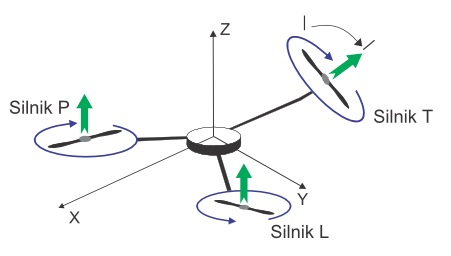
\includegraphics[width=0.7\linewidth]{./include/orientation}
\caption{Przyjęta orientacja tricoptera w układzie współrzędnych.}
\label{fig:orientation}
\end{figure}

Tricopter należy grupy rzadko spotykanych wielokomórkowców wyposażonych w nieparzystą liczbę silników odpowiadających za napędy w układzie.
Konstrukcja ta zdecydowanie utrudnia sterowanie ze względu na brak stabilności tego układu. Spowodowane jest to brakiem kompensacji siły bocznej pochodzącej od napędu niesparowanego. Czego skutkiem jest  efekt autorotacji obiektu wokół osi Z przy założeniu, iż wszystkie wirniki są w pozycji pionowej, tak jak w przypadku większości obiektów latających pionowego startu. Aby wyeliminować powyższy efekt zastosowano odpowiedni moduł składający się z serwomechanizmu, który reguluje kąt nachylenia wirnika T.


Przemieszczanie obiektu latającego w przestrzeni wymaga opracowania metodyki sterowania poszczególnymi wirnikami podczas przemieszczania się względem każdej z osi.
Bazując na poprzednim algorytmie sterującym zaprezentowano poniżej sposoby przemieszczania względem konkretnych osi tricoptera. Szczegółowe informacje związane z powyższymi zagadnieniami zostały opisane w pracy inżynierskiej autora w rozdziale 5. %TODO zrobic odnosnik do inz

\subsection{Przemieszczanie względem osi X}
Aby dokonać obrotu względem osi X konieczna jest ingerencja w ciąg wirników L oraz P. Aby uzyskać efekt przechylenia w lewą stronę konieczna jest redukcja siły ciągu na silniku L. Opcjonalnie w celu przyśpieszenia manewru można proporcjonalnie zwiększyć ciąg silnika P. Na rysunku \ref{fig:axis_x} przedstawiono opisany manewr.

\begin{figure}[!htbp]
\centering
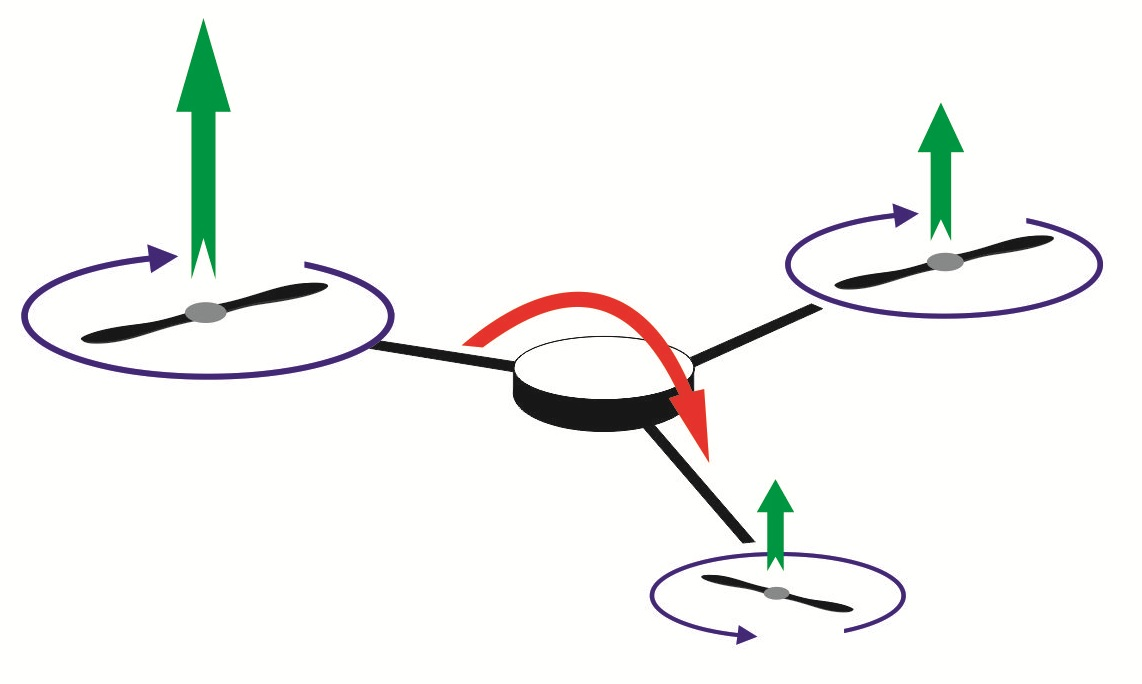
\includegraphics[width=0.7\linewidth]{./include/axis_x}
\caption{Sterowanie oraz stabilizacja w osi X.}
\label{fig:axis_x}
\end{figure}


\subsection{Przemieszczanie względem osi Y}
Obrót względem osi Y można zdecydowanie określić jako najważniejszy dla każdego obiektu latającego, odpowiada on za przemieszczenie się w przód. Odchylenie tricoptera zapewnia się przez regulację ciągu na wirniku T. Tak jak w przypadku osi X można zwiększyć prędkość obrotu obiektu przez symetrycznym modyfikacją mocy silników L oraz P wartość przeciwną co do znaku względem modyfikacji wirnika Z. Manewr ten został przedstawiony na rysunku \ref{fig:axis_y}.
\begin{figure}[!htbp]
\centering
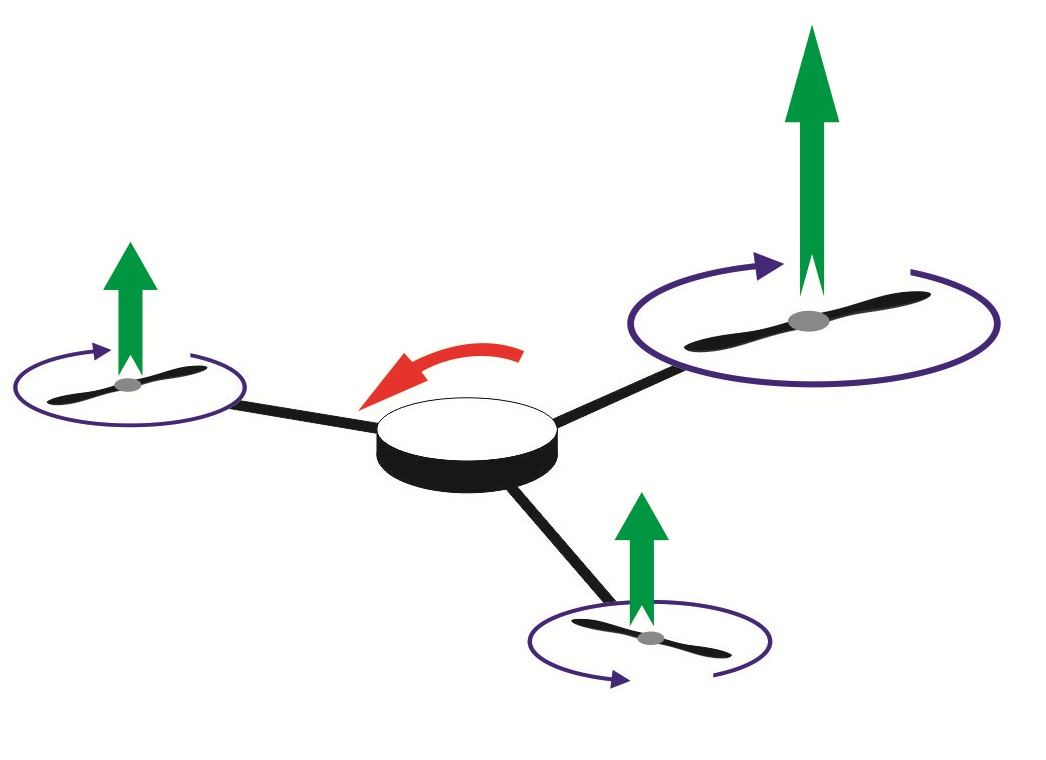
\includegraphics[width=0.7\linewidth]{./include/axis_y}
\caption{Sterowanie oraz stabilizacja w osi Y.}
\label{fig:axis_y}
\end{figure}


\subsection{Przemieszczanie względem osi Z}
Przemieszczanie względem osi Z jest głównie używane do zmiany kierunku lotu tricoptera. Manewr ten można wykonywać bez ingerencji w moc każdego z wirników. Zmiana kąta nachylenia silnika T powoduje pojawienie się efektu rotacji obiektu. Warto zwrócić uwagę, iż zbyt duże odchylenie wirnika od punktu stabilnego spowoduje również ruch tricoptera względem osi Y, ponieważ zmiana kąta nachylenia silnika Z powoduje zmianę pionowej siły ciągu, która odpowiada również za stabilizację tego obiektu. 

\begin{figure}[!htbp]
\centering
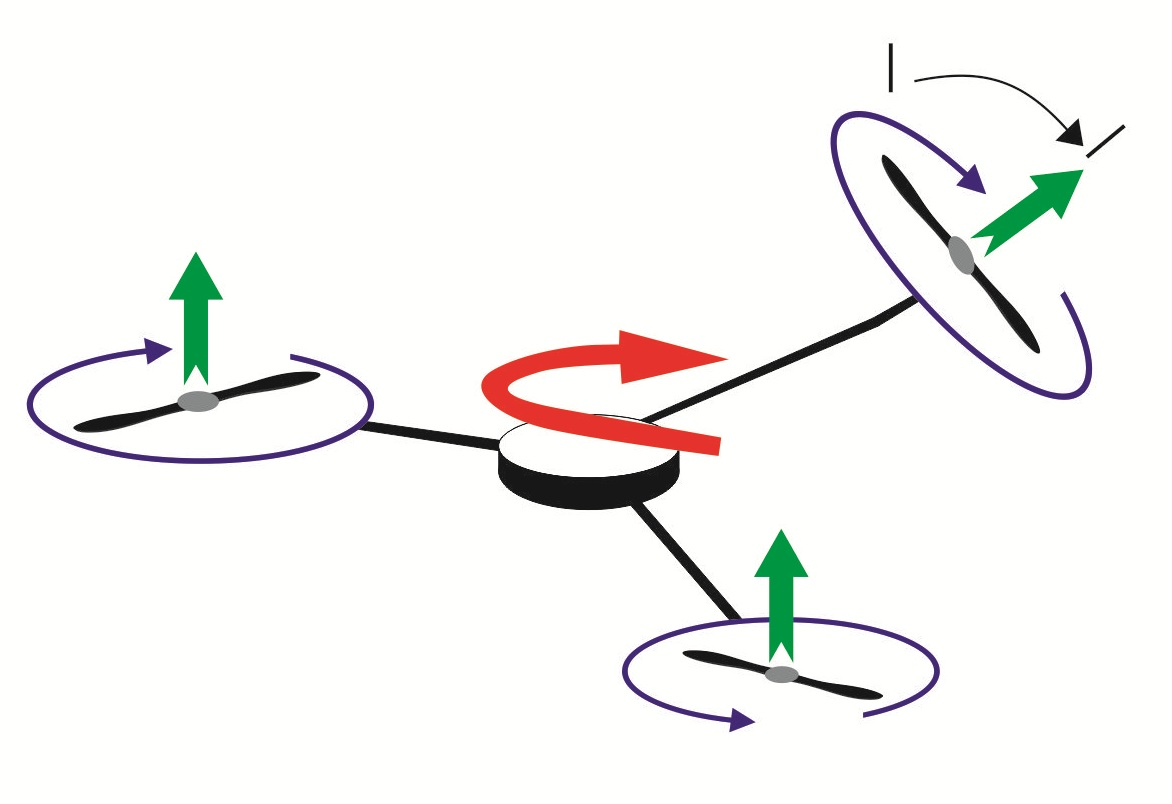
\includegraphics[width=0.7\linewidth]{./include/axis_z}
\caption{Sterowanie oraz stabilizacja w osi Z.}
\label{fig:axis_z}
\end{figure}


\section{Budowa modelu}
Ze względu na to, iż temat tej pracy bazuje na wykorzystaniu do testów gotowego obiektu latającego typu tricopter, autor zdecydował pominąć szczegółowy opis budowy modelu.
Szczegółowe informacje dotyczące konstrukcji oraz parametrów wielowirnikowca zostały przedstawione w pracy inżynierskiej autora w rozdziale 2. %TODO odnośnik do inż.






% itd.
% \appendix
% \include{dodatekA}
% \include{dodatekB}
% itd.

\bibliographystyle{alpha}
\bibliography{bibliografia}
%\begin{thebibliography}{1}
%
%\bibitem{Dil00}
%A.~Diller.
%\newblock {\em LaTeX wiersz po wierszu}.
%\newblock Wydawnictwo Helion, Gliwice, 2000.
%
%\bibitem{Lam92}
%L.~Lamport.
%\newblock {\em LaTeX system przygotowywania dokumentów}.
%\newblock Wydawnictwo Ariel, Krakow, 1992.
%
%\bibitem{Alvis2011}
%M.~Szpyrka.
%\newblock {\em {On Line Alvis Manual}}.
%\newblock AGH University of Science and Technology, 2011.cccccc
%\newblock \\\texttt{http://fm.ia.agh.edu.pl/alvis:manual}.
%
%\end{thebibliography}

\end{document}
